\documentclass{article}
\usepackage[utf8]{inputenc}
\documentclass[a4paper, 14pt]{article}
\usepackage{fancyhdr}
\usepackage[14pt]{moresize}
\usepackage[pdftex]{graphicx}
\usepackage{epstopdf}

\title{ME20B150.tex}
\author{Rithwin K Ashraf me20b150}
\date{June 2021}

\usepackage{epstopdf}
\pagestyle{empty}
\addtolength{\oddsidemargin}{-.95in}
\addtolength{\evensidemargin}{-.95in}
\addtolength{\textwidth}{1in}
\addtolength{\topmargin}{-0.85in}
\addtolength{\textheight}{1.5in}
\begin{document}
\begin{center}
	{\LARGE {\textbf {MM2090 ASSIGNMENT 4}}}
\end{center}

\section{Details}
\textbf {Name} : \textbf{\textit {Rithwin K Ashraf}}\\
\textbf {Roll No.} : \textbf{\textit {ME20B150}}\\
\textbf {Group} : \textbf{\textit {Group-1}}
\section{The Gravitational Force Equation}
\subsection{The Equation}
\begin{equation}
	{\LARGE{\textbf{$F =\frac{Gm1m2}{{r^2}}$}}}
	\label{eq:1}
\end{equation}
{\normalsize {The above given equation \ref{eq:1}  has terms \textbf{F} ,\textbf{G} , \textbf{m1},\textbf{m2} and \textbf{r}.}}

{\normalsize { Here,}\\
{\normalsize {\textbf{F} represents the force exerted by m1 on m2 or vice versa }}\\
{\normalsize {\textbf{G} \  represents the Gravitational Constant}}\\
{\normalsize {\textbf{m1} \  represents the mass of object1}}\\
{\normalsize {\textbf{m2} \  represents the mass of object2}}\\
{\normalsize{\textbf{r} \ represents the distance between object 1 and object2}}
\subsection{Description}

{\small {This is a general physical law derived from empirical observations by what Isaac Newton called inductive reasoning.}}

{\small {Newtons laws of universal gravitation(see equation \ref{eq:1}) is usually stated as that every particle attracts every other particle in the universe with a force that is directly proportional to the product of their masses and inversely proportional to the square of the distance between their centers.
\begin{figure}[h]
\centerline{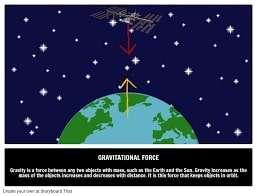
\includegraphics[scale=0.95]{me20b150.jpg}}
	\caption{Gravity\cite{fig}}
        \label{fig:1}
\end{figure}

This is a general physical law derived from empirical observations by what Isaac Newton called inductive reasoning.[4] It is a part of classical mechanics and was formulated in Newton's work Philosophiæ Natural is Principia Mathematica ("the Principia"), first published on 5 July 1687. When Newton presented Book 1 of the unpublished text in April 1686 to the Royal Society, Robert Hooke made a claim that Newton had obtained the inverse square law from him.
}}

{\small {Newton's law of gravitation resembles Coulomb's law of electrical forces, which is used to calculate the magnitude of the electrical force arising between two charged bodies. Both are inverse-square laws, where force is inversely proportional to the square of the distance between the bodies. Coulomb's law has the product of two charges in place of the product of the masses, and the Coulomb constant in place of the gravitational constant.


Webpage links\cite{webpage}
}}


%\bibliographystyle{plain}
%\bibliography{bibliography.bib}

\end{document}
